\documentclass{crypto-exercise}
\usepackage{hyperref}
\usepackage{tikz}
\usetikzlibrary{shapes,backgrounds}
\author{Sven Laur}
\contributor[Initial solution]{Raul-Martin Rebane}
\contributor[Streamlining]{Sven Laur}

\tags{Computational Diffie-Hellman problem, random self-reducibility}

\begin{document}
\begin{exercise}{Difference between random self-reducibility reductions of CDH}
  Let $\GG$ be a finite group of prime order $q$ such that all elements $y\in\GG$ can be
  expressed as powers of $g\in\GG$. Then the Computational
  Diffie-Hellman (CDH) problem is following. Given $x=g^a$ and
  $y=g^b$, find a group element $z=g^{ab}$. There are two well known ways 
  to reduce an instance of CDH to a random instance of CDH
  \begin{align*}
  &\begin{fblock}{\ADB(x,y)}
   &r,s\gets\ZZ_q\\
   &w\gets\AD(x\cdot g^r, y\cdot g^s)\\
   &z\gets \frac{w}{x^s \cdot y^r \cdot g^{rs}}\\
   &\RETURN z 
  \end{fblock}
  &
  &\begin{fblock}{\ADC(x,y)}
   &r,t\gets\ZZ_q, s\gets\ZZ_q^*\\
   &w\gets\AD(x\cdot g^r, y^s\cdot g^t)\\
   &z\gets\left(\frac{w}{x^t \cdot y^{rs} \cdot g^{rt}}\right)^{-s}\\
   &\RETURN z 
  \end{fblock}
  \end{align*}
  where $\AD$ is the algorithm designed to solve a random instance of CDH. Both of these
  algorithms can be used to amplify the success probability by majority voting. Analyse the success of both strategies
  \begin{align*}
   &\begin{fblock}{\ADB_n(x,y)}
   &\begin{forblock}{i\in\set{1,\ldots,n}}
     &r,s\gets\ZZ_q\\
     &w_i\gets\AD(x\cdot g^r, y\cdot g^s)\\
     &z_i\gets \frac{w_i}{x^s \cdot y^r \cdot g^{rs}}\\
   \end{forblock} \\
   &\RETURN \textsc{Majority}(z_1,\ldots,z_n) 
  \end{fblock}
  &
  &\begin{fblock}{\ADC_n(x,y)}
   &\begin{forblock}{i\in\set{1,\ldots,n}}
     &r,t\gets\ZZ_q, s\gets\ZZ_q^*\\ 
     &w_i\gets\AD(x\cdot g^r, y^s\cdot g^t)\\
     &z_i\gets\left(\frac{w_i}{x^t \cdot y^{rs} \cdot g^{rt}}\right)^{-s}\\
   \end{forblock} \\
   &\RETURN \textsc{Majority}(z_1,\ldots,z_n) 
  \end{fblock}
  \end{align*}
  by defining a sharp enough lower bound on the success probability. Sketch how the bound 
  behaves as a function of $n$. How big must $\ADVCDH{\GG}{\AD}$ be to get a noticeable 
  success probability?  
\end{exercise}
\begin{solution}
We divide the analysis into three distinct parts. First, we establish correctness. Second, we establish properties of the output distribution $z$. Third, we use established results together with standard probability bounds to lower and upper bound the success probability.

\vspace*{2ex}
\noindent\textsc{Correctness.}
Let $\alpha,\beta,\gamma$ be such that $x=g^\alpha$, $y=g^\beta$, $w=g^\gamma$ and $z=g^\delta$. 
Now if $\AD$ returns a correct answer then $\gamma=(\alpha+r)(\beta+s)$
in the algorithm $\ADB$ and $\gamma=(\alpha+r)(\beta s + t)$ in the algorithm $\ADC$. Consequently, 
\begin{align*}
\delta=(\alpha+r)(\beta+s) - \alpha s -\beta r-rs=\alpha\beta
\end{align*}  
in the algorithm $\ADB$ and
\begin{align*}
\delta s=(\alpha+r)(\beta s + t) - \alpha t -\beta rs -rt=\alpha\beta s
\end{align*} 
in the algorithm $\ADC$ and the reconstruction of $z$ is indeed successful.

\vspace*{2ex}
\noindent\textsc{Analysis of output distribution.}
First, note that additive noise component in both algorithms completely blinds inputs and thus $\AD$ receives a CDH random instance. 
The difference in the algorithm emerges if $\ADB$ gives a wrong answer. 
Let us assume that the answer of $\AD$ is offset by term $g^\epsilon$. Then the same offset propagates to the final answer in the algorithm $\ADB$ as
\begin{align*}
\delta=(\alpha+r)(\beta+s) + \epsilon - \alpha s -\beta r-rs=\alpha\beta + \epsilon\enspace.
\end{align*}  
In algorithm $\ADC$, the offset is randomised as  
\begin{align*}
\delta s=(\alpha+r)(\beta s + t) + \epsilon - \alpha t -\beta rs -rt=\alpha\beta s + \epsilon\enspace.
\end{align*} 
Since $\delta = \alpha\beta + \epsilon s^{-1}$ and $s$ is chosen uniformly from $\ZZ_q^*$, we get that $\delta$ is also uniformly distributed over $\ZZ_q\setminus\set{\alpha\beta}$ as the group size $q$ is a prime number by our assumptions. 
When the group size is not prime, the term $\epsilon s^{-1}$ may cycle through a proper subgroup of $\ZZ_q$ and thus the wrong answer is not converted into $q-1$ equiprobable values of $z$ rather there are fewer but still remarkable number of equiprobable values of $z$. 
The following allows to generalise the following results for groups where the order of group is a composite number but amplification is less powerful but such drop in efficiency is unavoidable.   


\vspace*{2ex}
\noindent\textsc{Success bounds for simple amplification strategy.}
Let us now analyse the algorithm $\ADB_n$.
The worst case for majority voting is where queries to $\AD$ gives either the correct answer or a wrong answer with constant offset $\epsilon$. 
Then the correct answer competes against single wrong answer and amplification is possible only if the probability of a correct answer $\ADVCDH{\GG}{\AD}>\frac{1}{2}$
Then we can encode the correct answer as  $1$ and the wrong answer as $0$ and view the majority voting process as a binomial distribution which yields $1$ with probability $\ADVCDH{\GG}{\AD} = \varepsilon$ and 0 with probability $1-\varepsilon$. The majority voting then yields the right answer if the sum of the trials is greater than $\frac{n}{2}$.
Let us recall that Hoeffding's inequality implies 
\begin{align*}
\pr{\sum_{i=1}^n X_i \leq (\varepsilon - \rho)n} \leq e^{-2\rho^2n}
\end{align*}
for independently drawn indicator variables $X_i\in\set{0,1}$ such that $\pr{X_i=1}=\varepsilon$.
Consequently, if we encode success of an $i$-th invocation of $\AD$ as the indicator $X_i$, we obtain an upper bound on the failure probability  
\begin{align*}
\pr{\ADB_n(g^\alpha,g^\beta)\neq g^{\alpha \beta}}= \pr{\sum_{i=1}^n X_i \leq \frac{n}{2}}\leq e^{-\frac{n(2\varepsilon-1)^2}{2}}
\end{align*}
that decreases exponentially wrt $n$. Note that the bound becomes effective only if $\varepsilon > \frac{1}{2}$. The same argument shows that amplification quickly converges to a wrong answer in the worst case scenario where $\AD$ always has a fixed offset $\delta$ for wrong answers and thus $\ADB_n$ is bound to fail when $\varepsilon < \frac{1}{2}$.
 
\vspace*{2ex}
\noindent\textsc{Success bounds for complex amplification strategy.}
Recall that by construction $z_i$ is a uniformly chosen among all possible answers that are wrong when $\AD$ fails. As a result, we can express 
\begin{align*}
\pr{z_i=g^{\alpha\beta+\epsilon}}&=
\begin{cases}
\varepsilon &\text{if } \epsilon=0\enspace,\\ 
\frac{1-\varepsilon}{q-1}    &\text{if } \epsilon\neq 0\enspace.\\ 
\end{cases}
\end{align*}
As the majority voting amplifies the probability of the most probable answer, the algorithm is applicable only if the probability of $z_i$ being correct is larger than a probability of any wrong value. From which we can conclude $\varepsilon >\frac{1}{q}$, i.e., when $\AD$ must work better than random guessing.   

Now note that correct answer can win only if the maximal number of wrong answers is at least one smaller than the number of correct answers. Let $F_{q-1,k}(\ell)$ denote the probability that when we sample $k$ values uniformly form $\ZZ_q^*$ maximal count of identical values is strictly smaller than $\ell$. Then we can decompose the probability of a correct answer as follows
\begin{align*}
\pr{\ADC_n(g^\alpha,g^\beta)=g^{\alpha\beta}}=
\sum_{\ell=2}^n\binom{n}{\ell}\varepsilon^\ell(1-\varepsilon)^{n-\ell}\cdot
F_{q-1,n-\ell}(\ell)
\end{align*}
as the first factor in the term corresponds to the probability that we obtain exactly $\ell$ correct answers and the second term corresponds to the probability that the remaining $n-\ell$ wrong answers do not overthrow the right verdict. For reasonable parameter values, the first term in the sum is the largest and thus we get a quite effective lower bound on the success:
\begin{align*}
\pr{\ADC_n(g^\alpha,g^\beta)=g^{\alpha\beta}}\geq
\frac{n(n-1)\varepsilon^2(1-\varepsilon)^{n-2}}{2}\cdot
F_{q-1,n-2}(2)
\end{align*} 
where the second probability $F_{q-1,n-2}(2)$ corresponds to the generalised birthday problem.

[Off by 1-F]

When the number of wrong answers $n-2\leq \sqrt{q-1}$ then the corresponding lower and upper bounds are quite tight: 
\begin{align*}
0.316\cdot
  \frac{(n-2)(n-3)}{q-1}\leq F_{q-1,k}(2)\leq 0.5\cdot
  \frac{(n-2)(n-3)}{q-1}\enspace.
\end{align*}
As there are generic algorithms for finding discrete logarithm in time $\Theta(\sqrt{q})$, the behaviour of the amplification algorithm is uninteresting for $n\geq \sqrt{q}$ and we do not have to consider bounds for the other ranges. 
Consequently, we can conclude
\begin{align*}
\pr{\ADC_n(g^\alpha,g^\beta)=g^{\alpha\beta}}\geq
0.158\cdot\frac{n(n-1)(n-2)(n-3)\varepsilon^2(1-\varepsilon)^{n-2}}{q-1}\cdot
\end{align*} 


  
 
The probability that all $n-2$ draws are distinct elements can  


To find the probability that at least two numbers are the same, we can use the findings of the generalized birthday problem.\footnote{\url{https://en.wikipedia.org/wiki/Birthday_problem\#Cast_as_a_collision_problem}} It has been shown that when drawing $n'$ random integers from a discrete uniform distribution with range $[1,d]$, the probability $P(n',d)$ that at least two numbers are the same is
\begin{center}
$P(n',d) \approx 1 - e^{\frac{-n'(n'-1)}{2d}}$
\end{center}
which in our case would be
\begin{center}
$P(n-2,|\GG|-1) \approx 1 - e^{\frac{-(n-2)(n-3)}{2(|\GG|-1)}}$
\end{center}
Thus $P(A \cap B) \approx (\frac{n(n-1)}{2} \varepsilon^2 (1-\varepsilon)^{n-2})  (1 - e^{\frac{-(n-2)(n-3)}{2(|\GG|-1)}})$
And the probability of $\ADC_n$ succeeding in this game is
\begin{center}
$P(A \setminus B) = P(A) - P(A \cap B) \approx \frac{n(n-1)}{2} \varepsilon^2 (1-\varepsilon)^{n-2} - (\frac{n(n-1)}{2} \varepsilon^2 (1-\varepsilon)^{n-2})  (1 - e^{\frac{-(n-2)(n-3)}{2(|\GG|-1)}}) = \frac{n(n-1)}{2} \varepsilon^2 (1-\varepsilon)^{n-2}e^{\frac{-(n-2)(n-3)}{2(|\GG|-1)}}$
\end{center}
Which gives us an approximate lower bound on the success of majority voting for $\ADC_n$. 

??

have less than $\ell$ coinciding values. 

us denote the probability  
\begin{align*}
F_{n}(\ell)=\pr{x??}
\end{align*} 
??

Let us first view a different game where instead of doing majority voting, $\ADC_n$ succeeds if he gets two right answers and there are no coinciding wrong answers. Note that the probability of success in this game is a lower bound on the probability of success in majority voting, as in majority voting $\ADC_n$ has more win conditions (for example 3 correct answers and 2 coinciding wrong answers). The probability that $\ADC_n$ outputs exactly two right answers is $\begin{pmatrix}
n \\
2
\end{pmatrix} \varepsilon^2 (1-\varepsilon)^{n-2} = \frac{n(n-1)}{2}\varepsilon^2 (1-\varepsilon)^{n-2} $. In the Venn diagram below, this is our probability of getting $A$, where we draw two right answers. $B$ stands for drawing two coinciding wrong answers. Our new game wins if we get $A \setminus B$. Thus we have to subtract the probability of getting $A \cap B$.


\begin{center}
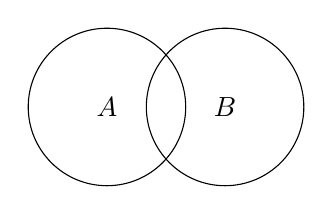
\begin{tikzpicture}
	\draw (0,0) circle (1cm) node {$A$};
	\draw (1.5,0) circle (1cm) node {$B$};
\end{tikzpicture}
\end{center}

To find $P(A \cap B)$ we can use the conditional probability formula $P(A \cap B) = P(A)P(B|A)$. $P(A) = \frac{n(n-1)}{2} \varepsilon^2 (1-\varepsilon)^{n-2}$ as above. $P(B|A)$ however stands for drawing at least two coinciding wrong answers, conditioned that we have drawn exactly two right answers. Since in this condition we have drawn two right answers, we have sampled the wrong answer distribution $n-2$ times. 

??


Example: Let's view the probability of winning this game in a setting where $\GG$ contains all 100 numbers and $\ADVCDH{\GG}{\AD} = \varepsilon = 0.2$. The probability of a fixed incorrect answer is then $\frac{0.8}{100-1}$. Figure \ref{approx} shows the approximate success probability of winning this game for a small range of $n$'s. We can see that at first we do get some amplification, for $n=8$, the probability of success is around $0.25$ which is an increase compared to $\varepsilon = 0.2$. However after that the success probability drops off. The reason for that is that the probability of two wrong answers coinciding is increasing significantly in that region, which causes loss in the game. However, in the majority voting case there will still be amplification going on, but to get a more accurate estimate of the amplification, we would have to view also the cases of reaching 3 or 4 correct answers with less coinciding wrong answers.

\begin{figure}[!htb]
\centering
%\includegraphics[width=\linewidth]{approximation.png}
\caption{Approximate probability of $\ADC_n$ succeeding in the game, $\varepsilon = 0.2$, $|\GG| = 100$}
\label{approx}
\end{figure}

??

For example, if $p = \ADVCDH{\GG}{\AD} = 0.55$, then $\varepsilon = 0.05$. Figure \ref{upperbound} illustrates lower bound on the probability that majority voting succeeds on a small range of $n$'s.
\begin{figure}[!htb]
\centering
%\includegraphics[width=0.45\linewidth]{hoeffding.png}
\caption{Lower bound on success ratio in given example $p = 0.55$, $\varepsilon = 0.05$}
\label{upperbound}
\end{figure}
Note that by using this bound we can compute the $n$ needed to find as high of a success probability as we want.


\end{solution}
\end{document}
